\documentclass[12pt]{report}

\usepackage[brazil,american]{babel}
\usepackage[utf8]{inputenc}
\usepackage[a4paper, total={6.5in, 9.5in}]{geometry}

\usepackage{titlesec}
\titleformat{\chapter}[display]
  {\normalfont\bfseries}{}{0pt}{\Huge}

\usepackage{url}
\usepackage{graphicx}
\usepackage{authblk}
\usepackage{hyperref}
\usepackage{lipsum}
\usepackage{xcolor}
\usepackage{float}

% \pagecolor[rgb]{0.1,0.1,0.1}
% \color[rgb]{0.9,0.9,0.9}

\begin{titlepage}
    \title{
        
\includegraphics[width=4cm]{img/logo.jpg} \\ 
        \large
        Dep. Ciência da Computação -- Universidade de Brasília (UnB)\\
        CIC0207 - Projeto Interdisciplinar de Licenciatura em Computação \\
        \vfill 
        \vfill
        \LARGE
        \textbf{Portal de Equações Matemáticas de Primeiro e Segundo Grau}
    }

    \author{
        Letícia Dias Soares Alves, 18/0022059\\
        Pedro Henrique de Brito Agnes, 18/0026305
    }
    
    \affil{
        \vfill
        \vfill
        \vfill
        Professora \\
        Dr.a Letícia Lopes Leite
    }

    \date{Brasília\\Novembro de 2020}

\end{titlepage}

\begin{document}
\maketitle

\selectlanguage{american}
\begin{abstract}
  With the great difficulty that can be observed on math students on school, it's necessary that they have access to some tools meant to help on the understanding of the subject and even awake their interest on it. To solve the problem, we have a portal of first and second degree equations in it's fist development stage which has as a goal, to help the students on learning the so feared subject that is used on many others, taking advantage of the interdisciplinarity with physics and chemistry among others.

  The portal have a basic explanation of the subject and a prototype of the page that will become a kind of calculator to help solving problems with equations. Every document related to the development of said website are also linked to it on a submenu.
\end{abstract}

\selectlanguage{brazil}
\begin{abstract}
  Com a grande dificuldade que pode ser observada nos estudantes em matérias de matemática, torna-se necessária a disponibilidade de ferramentas para o auxílio do ensino de forma melhorar o entendimento da matéria e até a despertar o interesse dos alunos. Para solucionar o problema, temos um portal de equações de primeiro e segundo grau na primeira fase de desenvolvimento que tem como objetivo, auxiliar os alunos no aprendizado desta matéria tão temida que é utilizada em diversas outras, tomando vantagem da interdisciplinaridade com a física, química e outros.

  O portal tem uma explicação básica do conteúdo e um protótipo de uma página que se tornará em um tipo de calculadora para auxiliar na resolução de questões. Todos os documentos também estão "linkados" em uma seção do submenu do portal.
\end{abstract}

\tableofcontents
\newpage

\chapter{Introdução}
Na matemática entendemos equação como, uma expressão algébrica que possui uma incógnita representada por uma letra (notações mais usadas são: x,y,z,w), e foi criada há muito tempo atrás para a solução de problemas quando o número é desconhecido. As equações de primeiro (onde o expoente da incógnita é igual a 1) e segundo grau  (onde o expoente da incógnita é igual a 2), desenvolvem um papel muito importante na rotina de alunos e professores, mas que muitas das vezes essas matérias acabam sendo passadas de forma tradicional e mecânica, que pode acabar interferindo na assimilação do conteúdo.

As equações são muito utilizadas no ensino fundamental (onde são ensinadas), caso o aluno não consiga assimilar a matéria, terá muitas dificuldades, pois, este mesmo conteúdo é usado no  nível médio e superior. Esse trabalho é desenvolvido com a finalidade de mostrar uma forma alternativa de passar esses conteúdos utilizando ferramentas que mostrem outras formas de apresentar a mesma matéria. Nossa ideia foi desenvolver um software onde o aluno possa escrever a equação desejada e ver a resolução da questão mostrando o passo a passo. 

\chapter{Problema}
É  comum atualmente muitos professores usarem metodologias tradicionais (onde o professor é o centro do processo de ensino aprendizagem), e isso acaba afetando todos os alunos que não conseguem se encaixar neste sistema. A tecnologia poderia auxiliar tanto os professores quanto os alunos, pois com o auxílio da tecnologia poderiam ser criadas muitas ferramentas para cada tipo de pessoa, alguns ferramentas com mais textos, imagens, vídeo aulas específicas, ou até mesmo jogos, questionários, etc.

A dificuldade na resolução de equações ao longo do período escolar é natural e se torna presente em muitos alunos, que acabam por perder todo o interesse pela matéria, em especial quando não conseguem encontrar uma aplicabilidade para elas. A baixa capacidade de resolução de equações pode afetar negativamente o desempenho em matérias como física, química e a própria matemática, em que este conteúdo é usado o tempo todo e qualquer pequeno erro já faz com que o aluno perca toda uma questão. O projeto tem como finalidade, a descomplicação do conteúdo por meio de um \textit{website}.

\chapter{Protótipo}
O software em desenvolvimento é, de certa forma inspirado no \href{https://pt.symbolab.com/}{Symbolab} e no Photomath que são "calculadoras" avançadas que mostram a resolução passo a passo dos exercícios desde os mais simples até os mais avançados com até matérias do ensino superior. O portal será composto de uma página com a explicação do conteúdo e outra com o modo de calculadora para a resolução de exercícios.

\section{Conteúdo}
A atual página principal do portal possui o início do que será a explicação do conteúdo, com exemplos de problemas resolvidos com a opção de clicar em cima para mostrar o passo a passo da resolução da equação se o usuário quiser tentar resolver antes por si só.

\begin{figure}[H]
    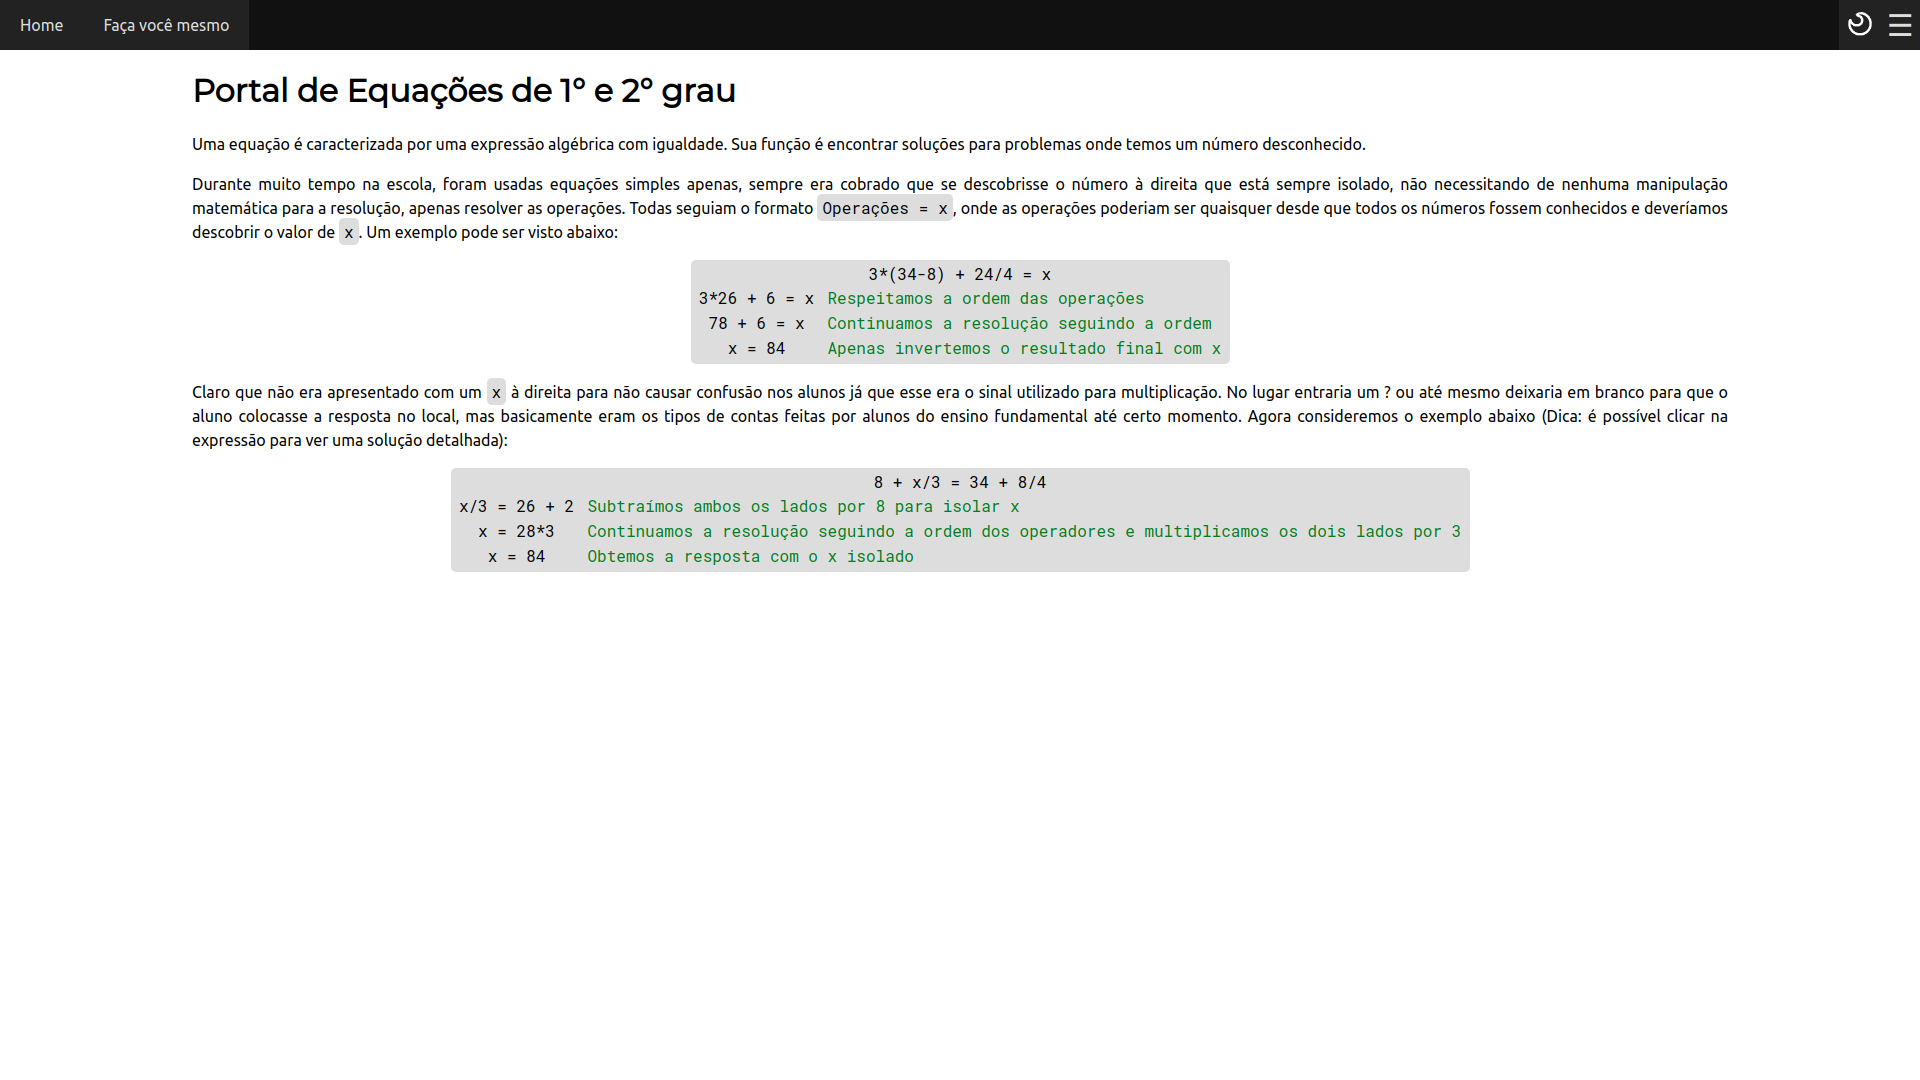
\includegraphics[width=1\textwidth]{img/home.png}
    \caption{Esboço da tela "Home" com as resoluções abertas}
\end{figure}

O portal atualmente possui um "dark mode" para agradar a todo tipo de público que pode ser ativado/desativado pelo botão na barra de navegação que tem um símbolo que lembra uma lua.

\begin{figure}[H]
    
\includegraphics[width=1\textwidth]{img/dark-mode.png}
    \caption{Esboço da tela "Home" com o modo escuro ativado e sem as resoluções dos exercícios abertas}
\end{figure}

Podemos ver na barra de navegação que temos outras opções também. Entre elas, mais à esquerda temos a "home", que é a página atual, ou seja, não servirá no contexto atual. Logo ao lado, temos a opção "Faça você mesmo" que é um link que leva à página que será usada para a resolução de exercícios informados pelo usuário. Mais à direita, temos o modo escuro como informado acima, e logo ao lado, temos um menu "sanduíche", que abre uma aba de navegação lateral para a inserção de outros links úteis.

\section{Exercícios}
Temos a segunda página que pode ser acessada pelo link informado acima "Faça você mesmo" que contém a seção de fazer os exercícios que podem ser informados pelo usuário. A tela consiste basicamente de um "input" de texto onde será informada uma equação e abaixo será mostrada a resposta ao clicar no botão.

\begin{figure}[H]
    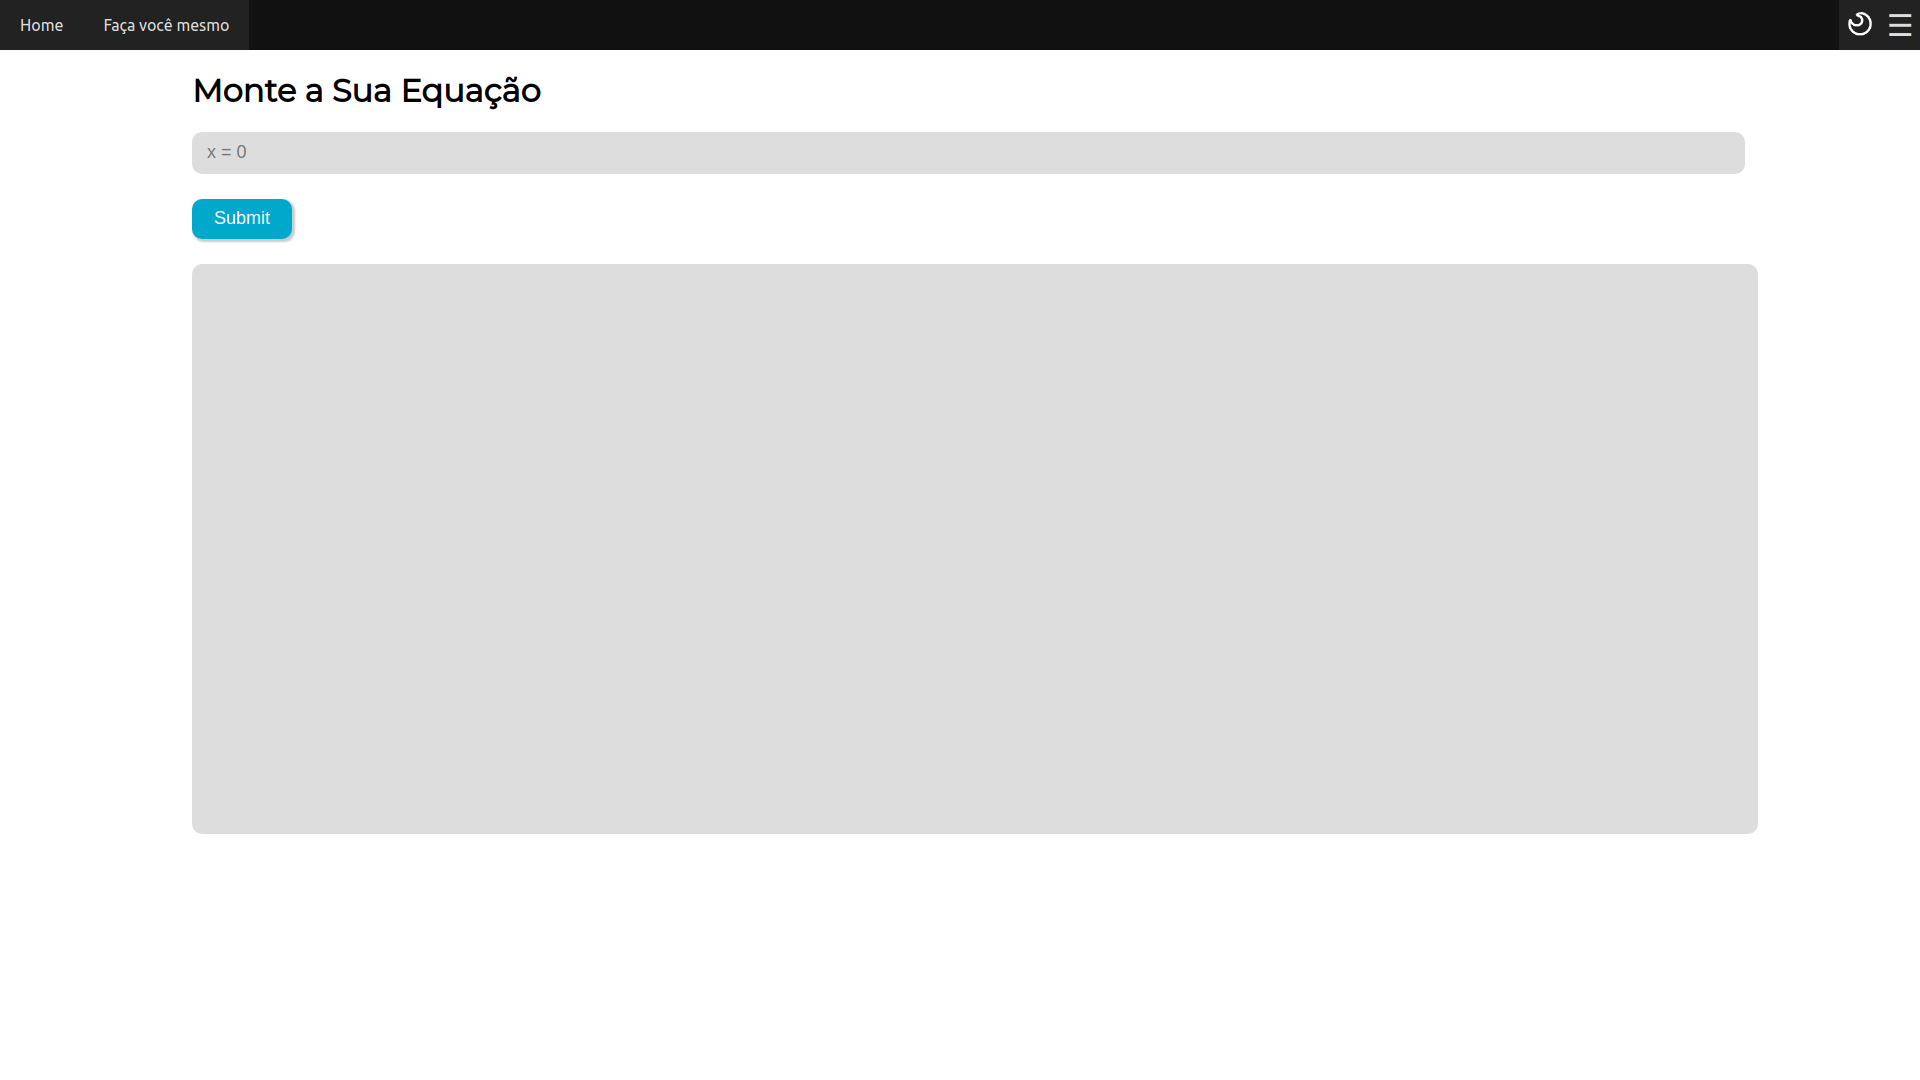
\includegraphics[width=1\textwidth]{img/interativo.png}
    \caption{Esboço da tela tela de exercícios}
\end{figure}

Assim como na página principal, o dark mode funciona nas demais páginas também, como é possível ver abaixo:

\begin{figure}[H]
    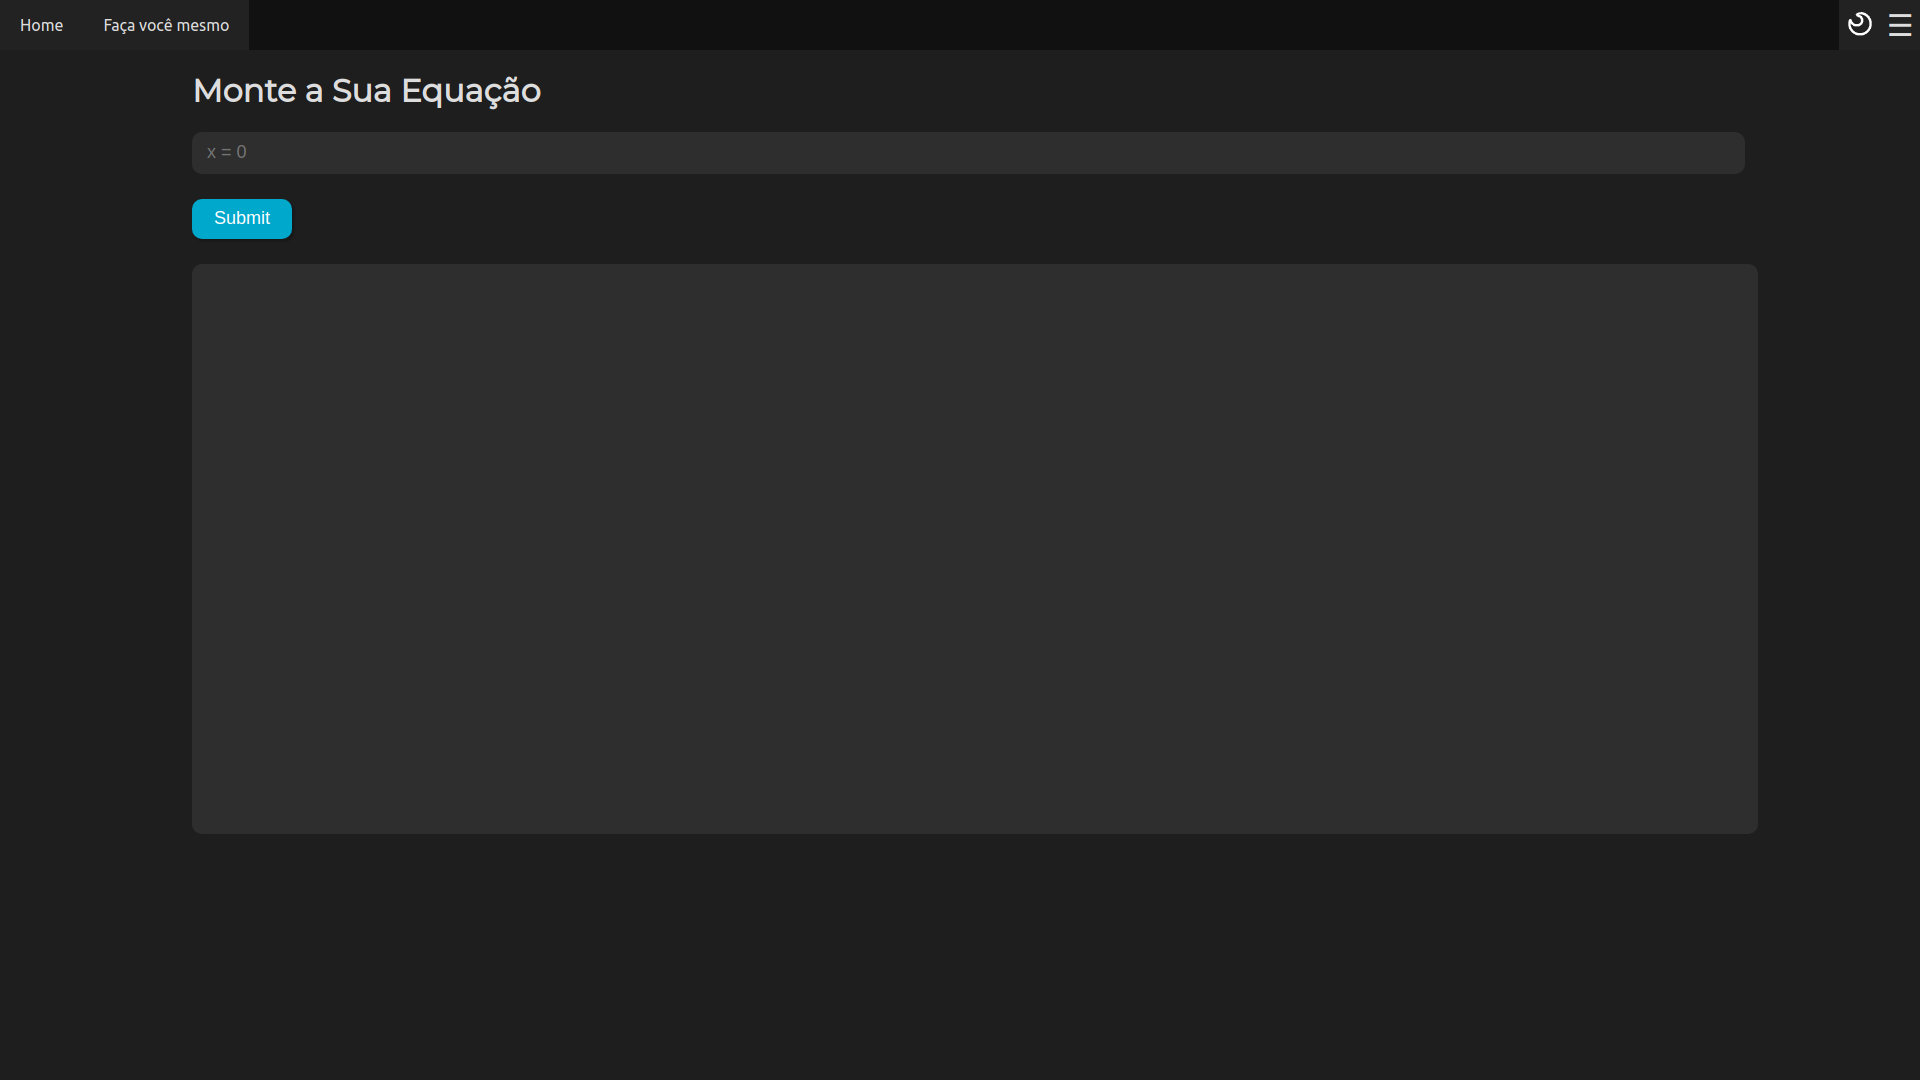
\includegraphics[width=1\textwidth]{img/interativo-dm.png}
    \caption{Esboço da tela de exercícios com o modo escuro ativado}
\end{figure}

Assim como na página principal, temos um submenu que pode ser acessado pelo ícone do "menu sanduíche", onde ficarão links úteis como este documento e o levantamento de requisitos.

\begin{figure}[H]
    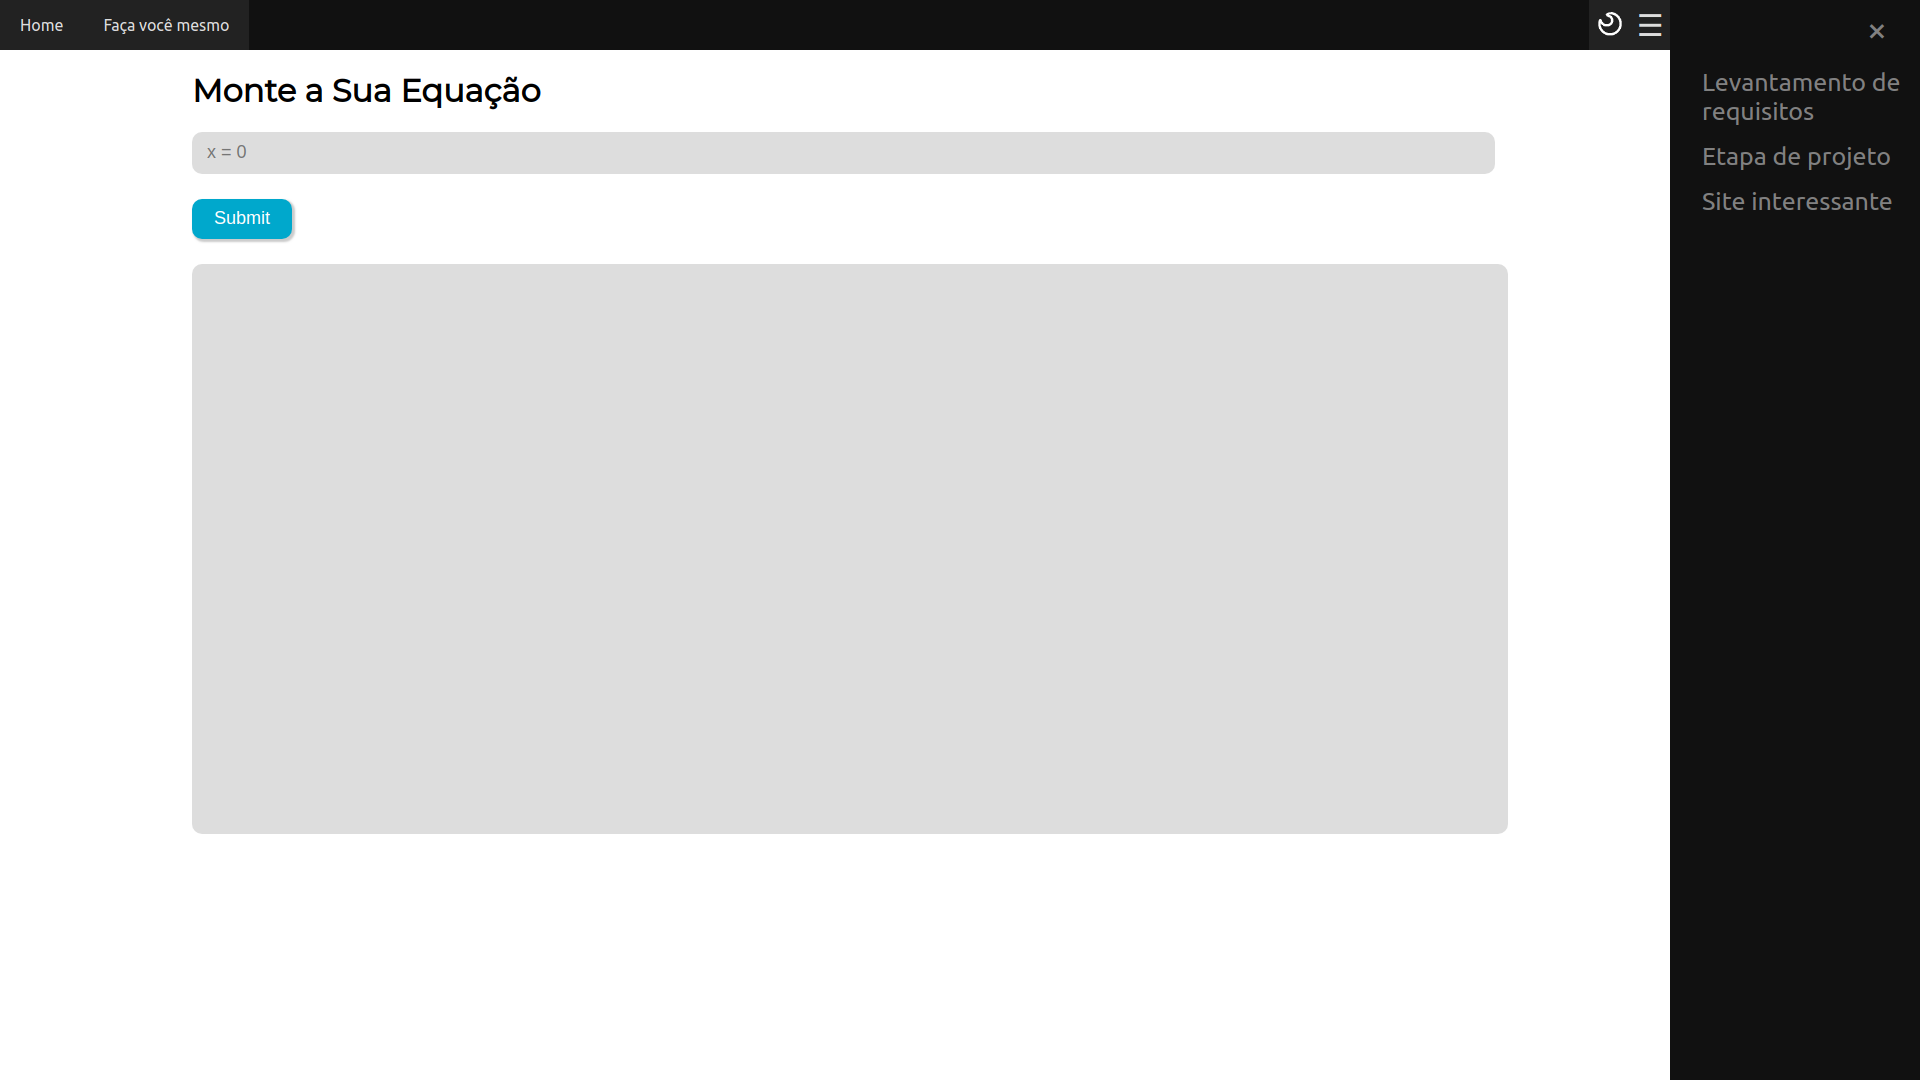
\includegraphics[width=1\textwidth]{img/submenu.png}
    \caption{Esboço da tela com o submenu lateral aberto}
\end{figure}

O portal está em desenvolvimento e poderá mudar com o tempo e até serem adicionadas novas páginas. O esboço atual é o básico do layout que o projeto seguirá. Para acessr a versão mais recente do portal, pode ser usado o seguinte link: \url{https://pedenite.github.io/PILC-eq/}.

\chapter{Conclusão}
Podemos perceber que cada aluno possui sua maneira de estudar e assimilar os conteúdos passados e com o auxílio das ferramentas tecnológicas cada pessoa pode escolher uma que ajude a entender a matéria mais facilmente.

\end{document}
